\documentclass{article}

\usepackage{graphicx}

\begin{document}
	\section*{Lab4 - Filip Jędrzejewski}
	
	\subsection*{Opis problemu}
	
	Celem zadania było wyznaczenie wielomianów interpolujących następujące funkcje:
	
	\begin{equation}
		f_1(x) = \frac{1}{1+25x^2} \quad  \quad x \in [-1,1]
	\end{equation}
	
	\begin{equation}
		f_2(x) = e^{\cos x} \quad  \quad x \in [0,2 \pi]
	\end{equation}
	
	używając: 
	
	\begin{itemize}
		\item Wielomianów Lagrange'a z równoodległymi węzłami
		\item Kubicznych funkcji sklejanych z równoodległymi węzłami
		\item Wielomianów Lagrange'a z węzłami Czebyszewa
		
		\begin{equation}
			x_j = cos(\theta_j) \quad , \quad \theta_j = \frac{2j+1}{2(n+1)}\pi
		\end{equation}
		przy czym $j = 0, 1, 2, ..., n$ 
			
	\end{itemize}
	
	\subsection*{Analiza funkcji $f_1(x)$}
	
	Dla funkcji $f_1(x)$ z $n=12$ węzłami interpolacji przedstawiono na wspólnym wykresie wyznaczone wielomiany interpolacyjne, funkcję sklejaną oraz węzły interpolacji.
	
	\begin{figure}[h]
    		\centering
  		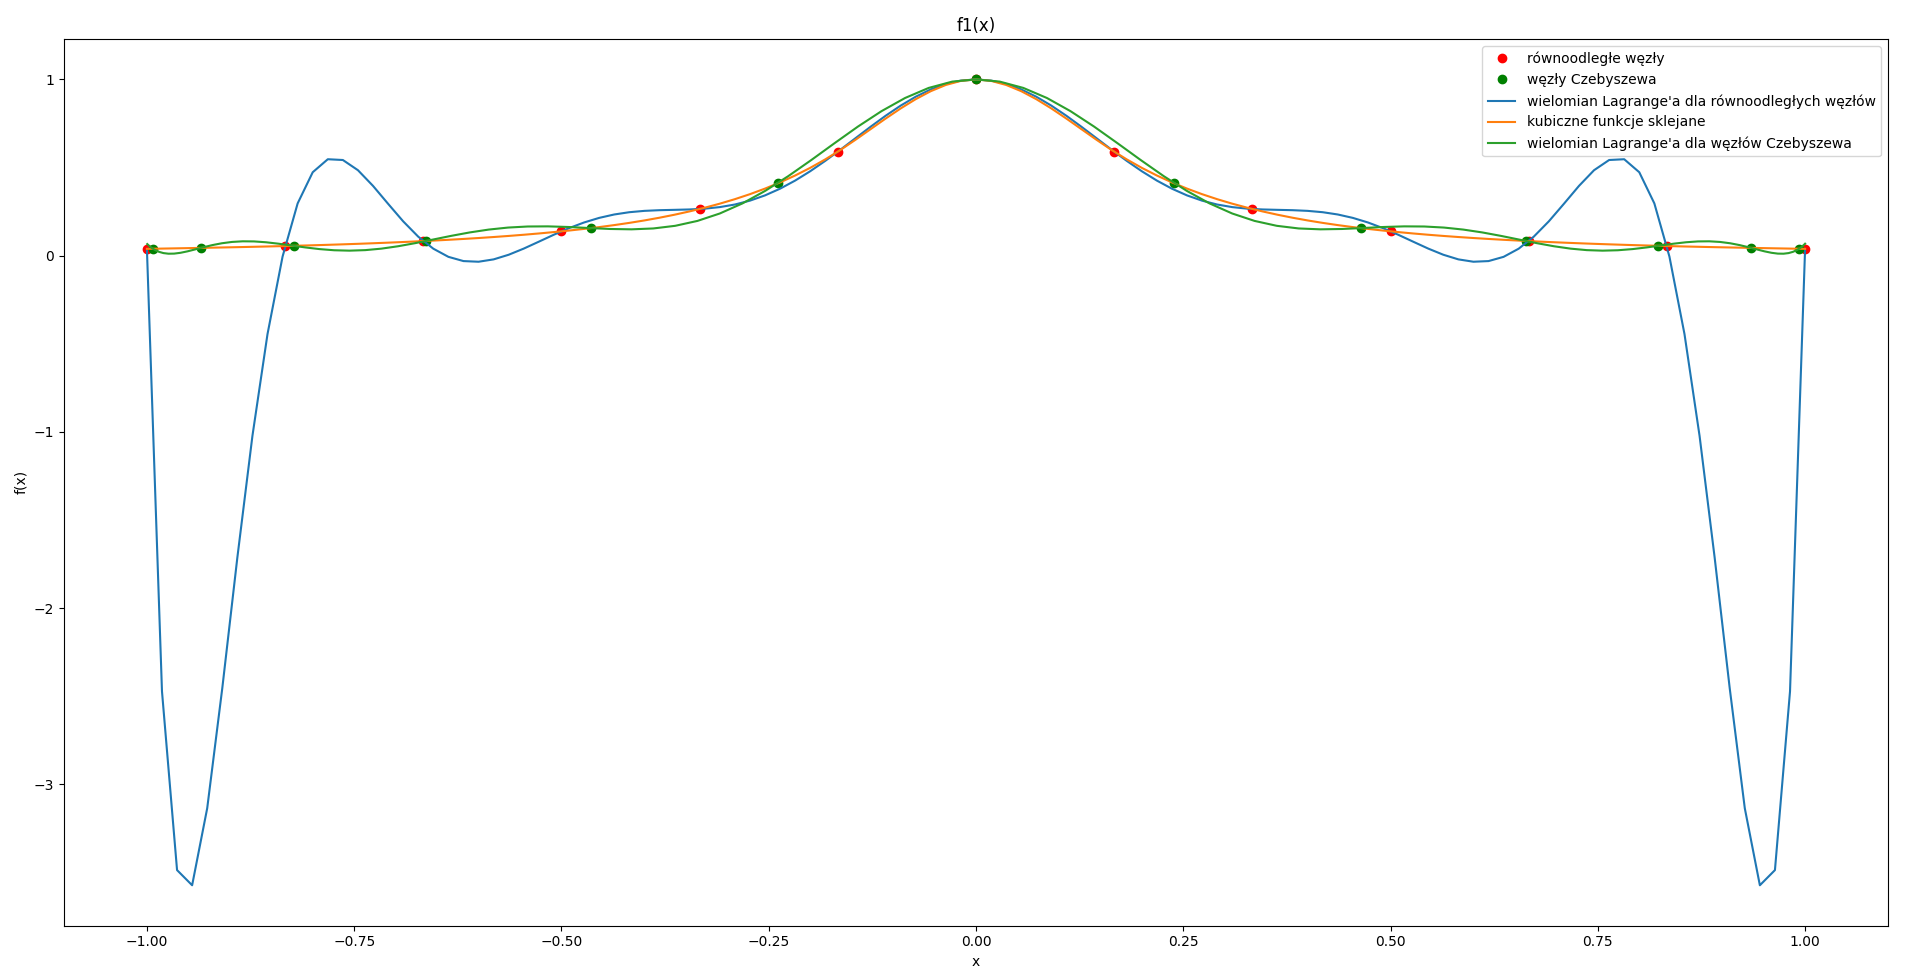
\includegraphics[scale = 0.3]{wykres1.png}
	\end{figure}
	
	Na wykresie można zauważyć, że wielomian Lagrange'a korzystający z równoodległych węzłów znacząco różni się od wielomianu Lagrange'a korzystającego z węzłów Czebyszewa albo funkcji sklejanej, szczególnie na brzegach przedziału.
	
	
	
	
	\subsection*{Wykresy błędów}
	
	Wykonano interpolację funkcji $f_1(x)$ i $f_2(x)$ dla $n = 4,5,...,70$ węzłów interpolacji, używając każdej z powyższych metod przybliżania funkcji. Dla $500$ losowo wybranych argumentów z dziedzin $f_1(x)$ oraz $f_2(x)$ wyznaczano wartości tych funkcji oraz ich przybliżeń. Na podstawie tych danych tworzono 500-wymiarowy wektor błędów, którego współrzędne były wyznaczane w następujący sposób:
	
	\begin{equation}
		a_i = f(x_i)-f_p(x_i)
	\end{equation}	 
	
	przy czym: $a_i$ - i-ta współrzędna wektora błędów, $f$ - przybliżana funkcja ($f_1$ lub $f_2$), $f_p$ - wyznaczone przybliżenie funkcji $f$, $x_i$ - wylosowana wartość z dziedziny funkcji $f$.	
	\newline \newline
	Jako całościowy błąd danego przybliżenia wybrano normę wektora błędu. Na podstawie tych danych wykonano wykresy błędu danego przybliżenia w zależności od liczby węzłów dla obu funkcji. Oś pionową wykresów przedstawiono w skali logarytmicznej ze wzgłędu na duże rozbieżności wartości błędów. \newline \newline
	Na wykresie dotyczącym funkcji $f_1$ można zauważyć, że wartość błędu w metodzie Lagrange'a dla równoodległych węzłów rośnie wraz ze wzrostem liczby węzłów. Jest to przykład efektu Rungego. Najbardziej dokładną metodą do przybliżania funkcji dla $n<50$ są kubiczne funkcje sklejane, natomiast dla $n>50$ najlepszą metodą jest interpolacja funkcji metodą Lagrange'a korzystająca z węzłów Czebyszewa. \newline \newline
	Na wykresie funkcji $f_2$ widzimy, że bezkonkurencyjnie najlepszą metodą przybliżania funkcji bez względu na liczbę węzłów $n$ jest interpolacja Lagrange'a z węzłami Czebyszewa. Dla $n<50$ najgorszą metodą są kubiczne funkcje sklejane, jednak ich skuteczność wraz ze wzrostem liczby węzłów rośnie (błąd maleje), natomiast początkowo malejący błąd interpolacji Lagrange'a z równoodległymi węzłami, dla $n>35$ zaczyna rosnąć (efekt Rungego) i dla $n>50$ staje się najmniej dokładną metodą przybliżania funkcji, stając się mniej dokładną niż kubiczne funkcje sklejane.
	
	
	\begin{figure}[h]
    		\centering
  		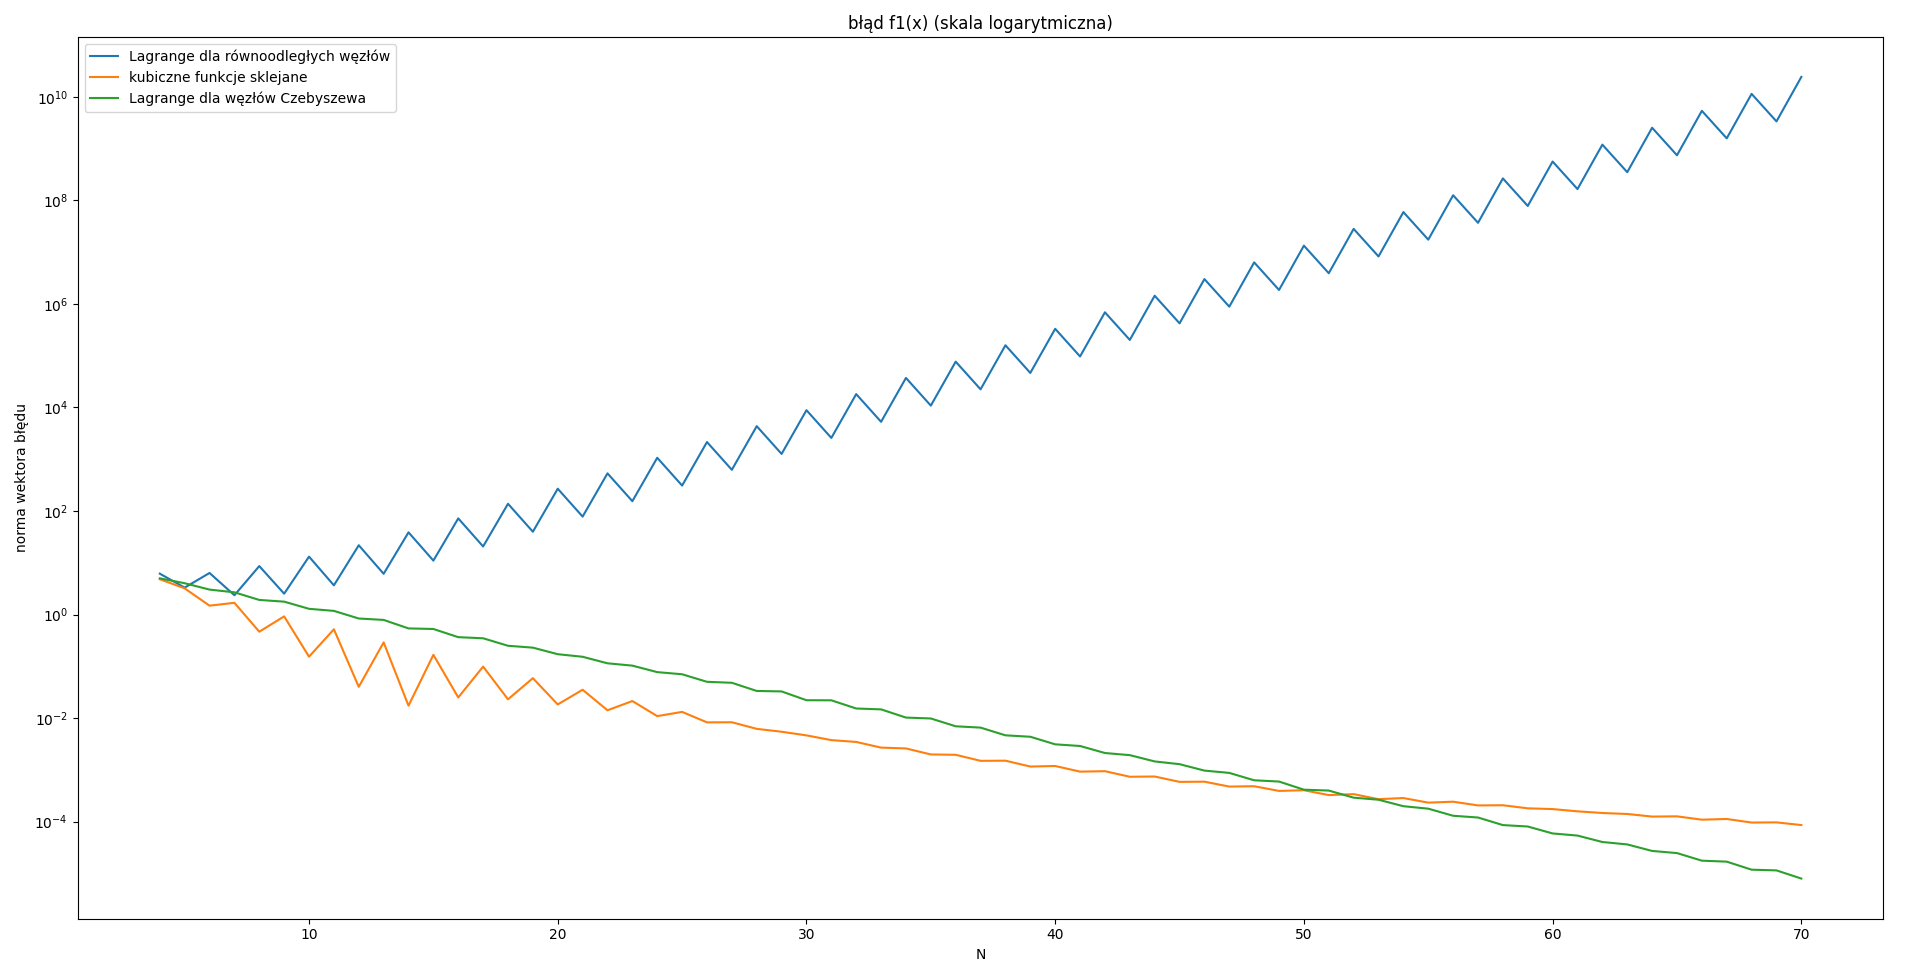
\includegraphics[scale = 0.3]{wykres2.png}
	\end{figure}
	
	\begin{figure}[h]
    		\centering
  		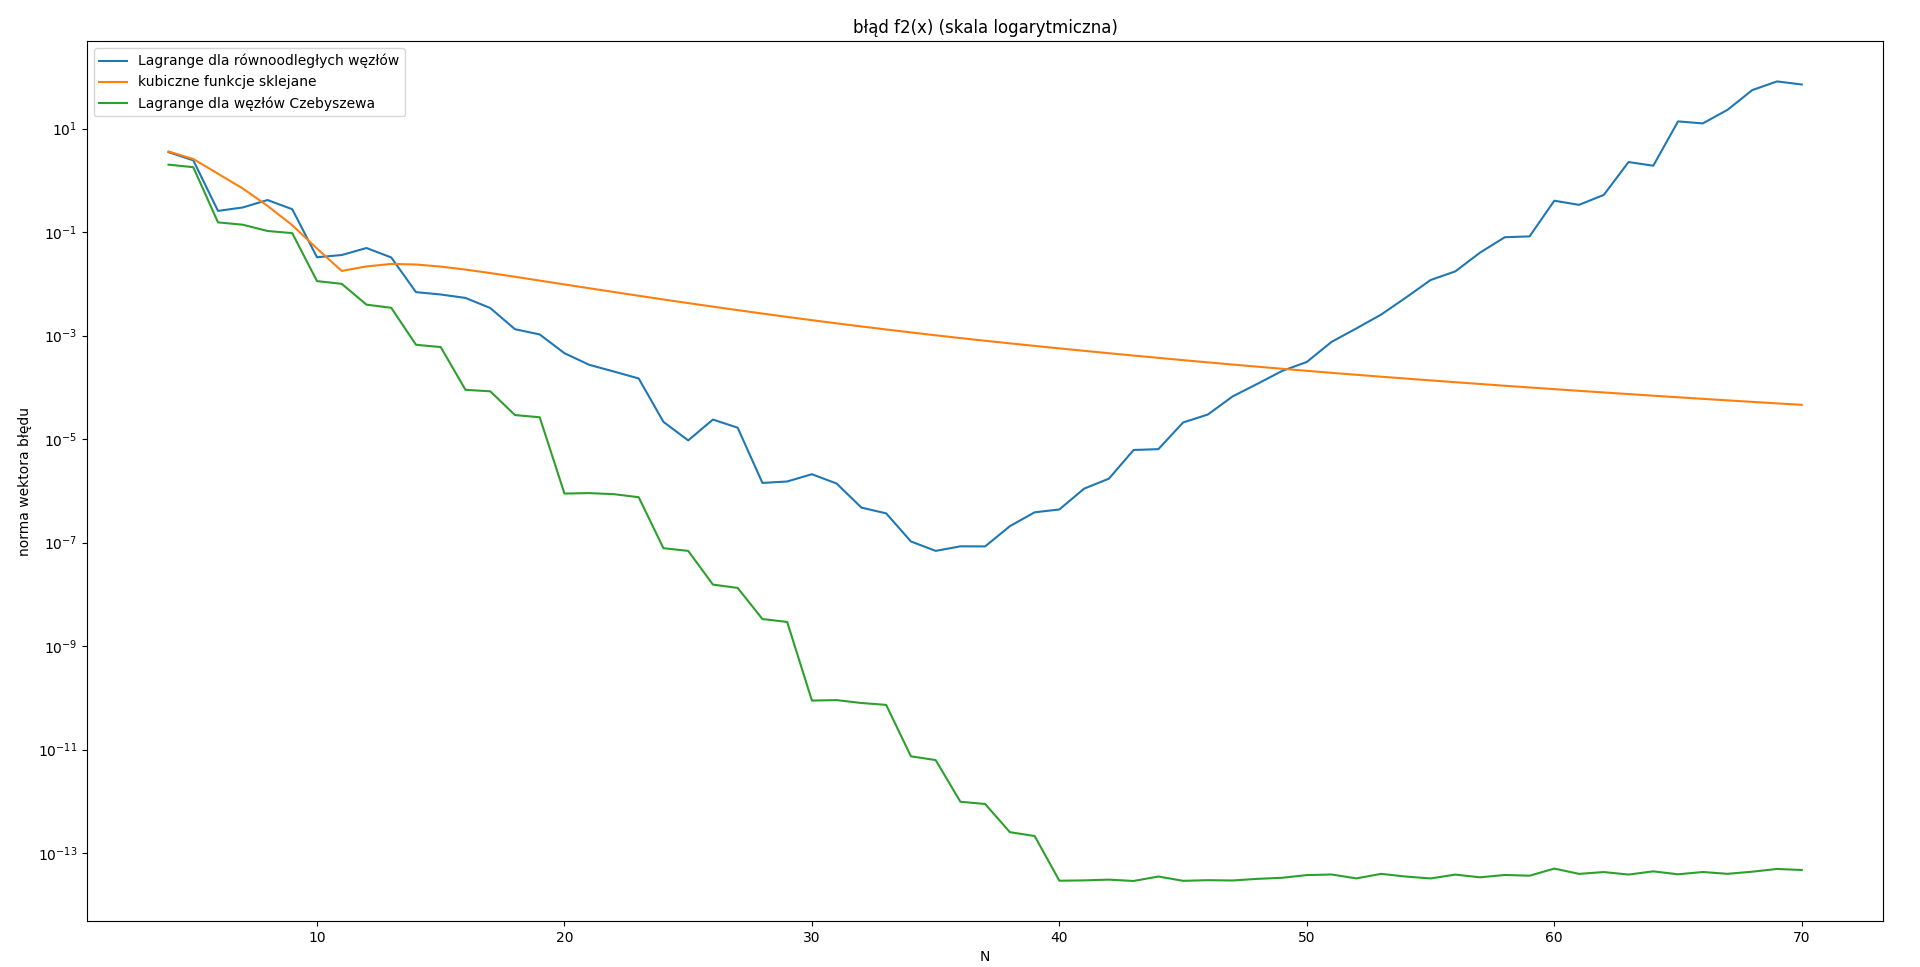
\includegraphics[scale = 0.3]{wykres3.png}
	\end{figure}
	
	
	
	
	
	
	
	
	
	
	
	
	
	
	
	
	
	
	
	
	
	
	
	
	
	
\end{document}